% !TEX root = main.tex
\documentclass[12pt]{beamer}
\usetheme{Boadilla}
\usefonttheme{default}
\usecolortheme{beaver}

% !TEX root = main.tex
% Mathematical symbols
\usepackage{amsmath,amsfonts,amssymb,amsthm,mathtools} % for formatting and enhancing mathematical notation and equations

% Images
\usepackage{graphicx} % for working with images
\graphicspath{{image/}}
\usepackage{tikz} % for creating graphics and diagrams directly 
\usetikzlibrary{calc}
\usepackage{floatrow} % provides additional control over figure and table placement, 
                      % including the [H] option for precise figure placement
\usepackage[margin=10pt,font=small,labelfont=bf,labelsep=period]{caption} % to configure 
                                    % the appearance of captions for figures and tables
%\usepackage{lipsum} % for generating placeholder text


% Tables
\usepackage{array} % for creating arrays and matrices within mathematical environments
\usepackage{tabularx} %  provides an environment for creating tables with columns of 
                      %  varying widths that automatically adjust to fit the content
\usepackage{tabulary} %  similar to the previous one
\usepackage{booktabs} %  enhancing readability and aesthetics
\usepackage{longtable} %  for creating tables that can span multiple page


\usepackage{hyperref} % for adding links and customizing them
\hypersetup{
	colorlinks=true,        % false: boxed links; true: colored links
	linkcolor=black,        % Color of internal links (e.g., table of contents)
	citecolor=refcolor,     % Color of citation links
	urlcolor=refcolor       % color of external links
}

\usepackage{biblatex} % bibliography-management package


%Custom colors
\definecolor{titlecolor}{RGB}{208,0,5}
\definecolor{refcolor}{RGB}{164,16,26} 
\definecolor{itemcolor}{RGB}{164,16,26}

\definecolor{foot1}{RGB}{240,166,166}
\setbeamercolor{color1}{fg=black,bg=foot1}

\definecolor{foot2}{RGB}{246,211,211}
\setbeamercolor{color2}{fg=black,bg=foot2}

\definecolor{foot3}{RGB}{240,223,223}
\setbeamercolor{color3}{fg=black,bg=foot3}

\definecolor{foot4}{RGB}{230,230,230}
\setbeamercolor{color4}{fg=black,bg=foot4}

%\definecolor{alertcolor}{RGB}{255,0,0} % Red for alerts
%\definecolor{boxcolor}{RGB}{0,128,0}  % Green for boxes
%\definecolor{examplecolor}{RGB}{0,0,255}  % Blue for example boxes


%Change colors
\setbeamercolor{titlelike}{parent=palette primary,fg=titlecolor}
\setbeamercolor{item}{fg=itemcolor}

%\setbeamercolor{alerted text}{fg=alertcolor}

%\setbeamercolor{block title}{bg=boxcolor, fg=white}
%\setbeamercolor{block body}{bg=white, fg=black}

%\setbeamercolor{block title example}{bg=examplecolor, fg=white}
%\setbeamercolor{block body example}{bg=white, fg=black}

%\setbeamercolor{block title alerted}{bg=alertcolor, fg=white} %
%\setbeamercolor{block body alerted}{bg=white, fg=black} 


%Footline
\setbeamertemplate{footline}{
\begin{beamercolorbox}[wd=\paperwidth,ht=2.25ex,dp=1ex,left]{color1}%
	\begin{beamercolorbox}[wd=0.3\paperwidth,ht=2.25ex,dp=1ex,center]{color1}%
		\insertshorttitle
	\end{beamercolorbox}%
	\begin{beamercolorbox}[wd=0.3\paperwidth,ht=2.25ex,dp=1ex,center]{color2}%
		\hspace*{5ex} \insertshortauthor
	\end{beamercolorbox}%
	\begin{beamercolorbox}[wd=0.3\paperwidth,ht=2.25ex,dp=1ex,center]{color3}%
		\hspace*{5ex} \insertshortdate
	\end{beamercolorbox}%
	\begin{beamercolorbox}[wd=0.1\paperwidth,ht=2.25ex,dp=1ex,center]{color4}%
		\hspace*{1ex} \insertframenumber{} / \inserttotalframenumber
	\end{beamercolorbox}%
\end{beamercolorbox}%
} 


% Define the \box and \myboxmath commands with the custom color
\usepackage{tcolorbox} 
\newtcbox{\mybox}{on line,colback=white,colframe=refcolor,size=fbox,arc=3pt,boxrule=0.8pt}
\newcommand{\myboxmath}[1]{\mybox{$#1$}}


%The next block of commands puts the table of contents at the 
%beginning of each section and highlights the current section:
\AtBeginSection[]
{
  \begin{frame}
    \frametitle{Table of Contents}
    \tableofcontents[currentsection]
  \end{frame}
}

% Remove the navigation bar from slides
\beamertemplatenavigationsymbolsempty 
% Enable numbering of figures and tables in captions
\setbeamertemplate{caption}[numbered]


\addbibresource{include/references.bib} % Import the bibliography file

\begin{document}

% !TEX root = main.tex

\title[Binarized NN MaxSAT]{Training Binarized NN with MaxSAT}
\subtitle{Knowledge and Representation Learning}
\author[Anna Putina]{Anna Putina\inst{1}}

\institute[Padua]
{
  \inst{1}%
  Università degli Studi di Padova
}

\date[February, 2025] 
{February, 2025}

\logo{
\includegraphics[height=1cm]{image/unipdlogo}}





%The next statement creates the title page
\frame{\titlepage}

%---------------------------------------------------------
%This block of code is for the table of contents after
%the title page
\begin{frame}
    \frametitle{Table of Contents}
    \tableofcontents
    \end{frame}
    
%---------------------------------------------------------
\section{Introduction}
\begin{frame}{Binarized Neural Networks}
\vspace{-0.2cm}
\begin{itemize}
    \item Neural networks with binary (\{-1,1\}) inputs, outputs, and weights.
    \item The goal is to find the set of weights that maximize the correct predictions of the net.
\end{itemize}
\vspace{-0.2cm}
\begin{figure}[H]
        \centering
        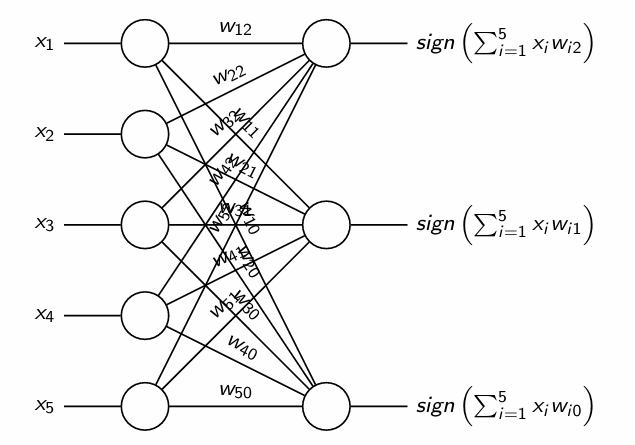
\includegraphics[height=0.55\textheight]{image/bnn}
        \caption{Binarized NN Structure}
    \end{figure}
\end{frame}


\begin{frame}{Objectives}
Fit a binarized neural network using MaxSAT:
\begin{enumerate}
    \item Implement a method to encode a binarized neural network layer with  \( m \) inputs and \( n \) outputs in Max-SAT.
    \item Use this method to encode an entire BNN with multiple stacked layers in Max-SAT.
    \item Define a training approach for the BNN using Max-SAT.
    \item Generate train/test data for three binary functions (5 inputs, 5 outputs) and evaluate different network configurations.
\end{enumerate}
\end{frame}


%---------------------------------------------------------
\section{Data Generation}

\begin{frame}
\frametitle{Dataset Creation}
\begin{itemize}
    \item The dataset consists of all possible binary input combinations of size N=5, where each input is either -1 or 1.
    \item The outputs are generated using different logical functions, allowing for varying levels of complexity.
\end{itemize}
\end{frame}

\begin{frame}
\frametitle{Logical Functions}
\begin{itemize}
    \item Three different logical functions are defined. Each function uses basic logical operations (AND, OR, XOR, NOT).
    \item Nested conditions that simulate real-world nonlinear relationships. The functions are designed to test the ability of the BNN to approximate logical structures.
\end{itemize}
\end{frame}

\begin{frame}{Logical Functions Example}
\vspace{-0.9cm}

\[
\text{logical\_function\_1}(x) =
\left\{
\begin{array}{c}
    (x_3, \quad x_1 \lor x_2, \quad x_0, \quad \neg x_3, \quad x_3 \land x_4)
\end{array} 
\right\}
\]

\vspace{-0.7cm}

\[
\text{logical\_function\_2}(x) =
\left\{
\begin{array}{c}
    (x_0 \land x_1, \quad x_2 \lor x_3, \\
    \quad (x_2 \land \neg x_3) \lor (\neg x_2 \land x_3), \quad \neg x_3, \\
    (x_4 \land x_0) \lor x_1)
\end{array}
\right\}
\]

\[
\text{logical\_function\_3}(x) =
\left\{
\begin{array}{c}
    ((x_0 \land x_1) \lor ((x_2 \land \neg x_3) \lor (\neg x_2 \land x_3))), \\
    (x_1 \lor x_2) \land (\neg x_3 \lor x_4), \\
    x_0 \lor (x_1 \land x_2 \land \neg x_3) \lor (\neg x_1 \land \neg x_2 \land x_3), \\
    (x_3 \land x_4) \lor (\neg x_0 \land \neg x_1) \lor (x_0 \land x_1), \\
    ((x_2 \land x_3) \lor (x_4 \land \neg x_0) \lor (\neg x_4 \land x_0)) \land x_1
\end{array}
\right\}
\]
\end{frame}


%---------------------------------------------------------
\section{SAT Encoding}

\begin{frame}
\frametitle{Indexing Scheme}
\begin{itemize}
    \item A single-layer BNN consists of:
    \begin{itemize}
        \item \( N \) input neurons
        \item \( M \) output neurons
        \item A weight matrix \( W \) of shape \( (N, M) \)
    \end{itemize}
    \item A multi-layer BNN consists of:
    \begin{itemize}
        \item \( N \) input neurons
        \item \( H \) hidden neurons
        \item \( M \) output neurons
        \item Two weight matrices:
        \begin{itemize}
            \item \( W_1 \) of shape \( (N, H) \) (input to hidden)
            \item \( W_2 \) of shape \( (H, M) \) (hidden to output)
        \end{itemize}
    \end{itemize}
    \item We assign unique indices to neurons and weights to avoid overlap in MaxSAT.
\end{itemize}
\end{frame}

\begin{frame}
\frametitle{General SAT Indexing Formula}
\begin{block}{SAT Indexing Function}
\begin{equation*}
    \text{SAT\_index}(i, n, N, \text{offset}) = \text{offset} + i \cdot N + n + 1
\end{equation*}
\end{block}
\begin{itemize}
    \item \( i \) - Current index (e.g., training sample).
    \item \( n \) - Neuron or weight index in a layer.
    \item \( N \) - Number of elements in the layer.
    \item \textbf{offset} - Used to distinguish different sections.
\end{itemize}
\end{frame}

\begin{frame}
\frametitle{Encoding Input Neurons}
\begin{block}{Input Encoding Formula}
\begin{equation*}
    x_{\text{enc}}(i, n) = \text{SAT\_index}(i, n, N, 0) = i \cdot N + n + 1
\end{equation*}
\end{block}
\begin{itemize}
    \item \( N \) - Number of input neurons.
    \item \( n \) - Index of an input neuron.
    \item \( i \) - Index of a training sample.
\end{itemize}
\end{frame}

\begin{frame}
\frametitle{SAT Index for First Layer Weights}
\begin{block}{Formula}
\centering
\begin{equation*}
    w_{1 \text{enc}}(i, h) = \text{SAT\_index}(n, h, H, \text{train\_size} \times N) = \\
    
    \text{train\_size} \times N + (n \times H) + h + 1
\end{equation*}
\end{block}
\begin{itemize}
    \item train\_size - Number of training samples.
    \item \( N \) - Number of input neurons.
    \item \( H \) - Number of hidden neurons.
    \item \( n \) - Index of an input neuron.
    \item \( h \) - Index of a hidden neuron.
\end{itemize}
\end{frame}

\begin{frame}
\frametitle{SAT Index for Second Layer Weights}
\begin{block}{Formula}
\centering
\begin{equation*}
    w_{2 \text{enc}}(h, m) = \text{SAT\_index}(h, m, M, \text{train\_size} \times N + N \times H) = \\
    \text{train\_size} \times N + (N \times H) + (h \times M) + m + 1
\end{equation*}
\end{block}
\begin{itemize}
    \item train\_size - Number of training samples.
    \item \( N \) - Number of input neurons.
    \item \( H \) - Number of hidden neurons.
    \item \( h \) - Index of a hidden neuron.
    \item \( M \) - Number of output neurons.
    \item \( m \) - Index of an output neuron.
\end{itemize}
\end{frame}


%---------------------------------------------------------
\section{Constraints}

\begin{frame}{Hard Constraints in MaxSAT}
\begin{itemize}
    \item Hard constraints are derived directly from the training data.
    \item Each input variable \( x_i^{(n)} \) is assigned a unique SAT index.
    \item A constraint holds True when \( x_i^{(j)} = 1 \) and False when \( x_i^{(j)} = -1 \).
\end{itemize}
\end{frame}

\begin{frame}{Activation Function Transformation}
\begin{itemize}
    \item Activation fucntion is $\text{sign}\left(\sum x_i w_i\right)$
    \item We use use the majority rule:
    \[ \left\{ \# x_i w_i > 0 \right\} \quad >  \quad \left\{ \# x_i w_i < 0 \right\} \] 
    \item $x, w \in \{-1,1\}$, thus $x_i w_i$ is equivalent to $x_i \equiv w_i$.

    \vspace{0.4cm}
    
    \textit{"\( x_i \equiv w_i \) for at least more than half the \( i \)'s."}

    \item This leads to the soft constraints: penalizing for misclassification.
    
\end{itemize}
\end{frame}

\begin{frame}{Activation Function as a logic formula}
\begin{itemize}
    \item Example for \( i = 1,2,3 \) for the postive output neuron.
\end{itemize}
\vspace{-0.6cm}

\centering

\[
(\neg x_1 \vee w_1)  \wedge (\neg w_1 \vee x_1) \wedge
(\neg x_2 \vee w_2)  \wedge (\neg w_2 \vee x_2)
\]

\vee

\[
(\neg x_1 \vee w_1)  \wedge (\neg w_1 \vee x_1) \wedge
(\neg x_3 \vee w_3)  \wedge (\neg w_3 \vee x_3)
\]

\vee

\[
(\neg x_2 \vee w_2)  \wedge (\neg w_2 \vee x_2) \wedge
(\neg x_3 \vee w_3)  \wedge (\neg w_3 \vee x_3)
\]

\end{frame}

\begin{frame}{Activation Function in CNF}
\begin{itemize}
    \item After transformation to CNF:
\end{itemize}

\vspace{-0.4cm}

\centering

\[
(x_1 \vee x_2 \vee \neg w_1 \vee \neg w_2) \wedge 
(x_1 \vee \neg x_2 \vee \neg w_1 \vee w_2) \wedge 
\]
\[
(\neg x_1 \vee x_2 \vee w_1 \vee \neg w_2) \wedge 
(\neg x_1 \vee \neg x_2 \vee w_1 \vee w_2)
\]

 \wedge 
\vspace{-0.8cm} 

\[
(x_1 \vee x_3 \vee \neg w_1 \vee \neg w_3) \wedge 
(x_1 \vee \neg x_3 \vee \neg w_1 \vee w_3) \wedge 
\]
\[
(\neg x_1 \vee x_3 \vee w_1 \vee \neg w_3) \wedge 
(\neg x_1 \vee \neg x_3 \vee w_1 \vee w_3)
\]

 \wedge 
 \vspace{-0.8cm}

\[
(x_2 \vee x_3 \vee \neg w_2 \vee \neg w_3) \wedge 
(x_2 \vee \neg x_3 \vee \neg w_2 \vee w_3) \wedge 
\]
\[
(\neg x_2 \vee x_3 \vee w_2 \vee \neg w_3) \wedge 
(\neg x_2 \vee \neg x_3 \vee w_2 \vee w_3)
\]
\end{frame}

%---------------------------------------------------------
\section{Complexity Analysis}

\begin{frame}{Computational Complexity with Hidden Layers}
\begin{itemize}
    \item Introducing a hidden layer significantly increases computational complexity.
    \item In a single-layer network, outputs are determined directly from input neurons and their corresponding weights.
    \item With a hidden layer, the output depends on:
    \begin{itemize}
        \item The activation of hidden neurons, influenced by input values and weights \( w^1 \).
        \item The combination of hidden neurons and their connections to output neurons via weights \( w^2 \).
    \end{itemize}
    \item This leads to exponential growth in the number of constraints required for encoding in CNF.
\end{itemize}
\end{frame}

\begin{frame}{Computational Complexity Example}
In the implementation case:
\begin{itemize}
    \item With N = 5 input neurons, M = 5 output neurons and \\
    train\_size = 22 training samples we have 8800 soft constraints.
    \item With N = 5 input neurons, H = 3 hidden neurons, M = 3 output neurons (the situation with 5 outputs is unfeasible for 15 Gb RAM computer) and train\_size = 22 training samples we have 5068800 soft constraints.
\end{itemize}
\end{frame}


%---------------------------------------------------------
\section{Results}

\begin{frame}{Experimental Results}
\begin{itemize}
    \item The dataset was split into 70\% for training and 30\% for testing.
    \item We compare a BNN without a hidden layer and a BNN with a hidden layer.
    \item The BNN without a hidden layer fails to handle even simple cases due to non-linearity of the logical functions.
    \item The BNN with a hidden layer achieves perfect training accuracy and high test accuracy but at a higher computational cost.
       \item Increasing the output neurons to 5 made training unfeasible, highlighting the scalability challenge of the MaxSAT approach.
\end{itemize}
\end{frame}

\begin{frame}{Experimental Results}
\begin{table}[H]
    \centering
    \begin{tabular}{|c|c|c|c|}
        \hline
        \textbf{Model} & \textbf{Solver Cost} & \textbf{Training Accuracy} & \textbf{Test Accuracy} \\ 
        \hline
        \multicolumn{4}{|c|}{\textbf{BNN Without Hidden Layer}} \\
        \hline
        Function 1 & 27 & 0.75 & 0.54 \\
        Function 2 & 27 & 0.75 & 0.54 \\
        Function 3 & 26 & 0.76 & 0.52 \\
        \hline
        \multicolumn{4}{|c|}{\textbf{BNN With Hidden Layer}} \\
        \hline
        Function 1 & 2 & 1.00 & 0.80 \\
        Function 2 & 4 & 1.00 & 0.80 \\
        Function 3 & 1 & 1.00 & 0.80 \\
        \hline
    \end{tabular}
    \caption{Comparison of BNN with and without a hidden layer}
\end{table}
\end{frame}

\end{document}